\section{Experimental Design}
\label{sec:design}

\subsection{Preliminary Three-Tier Study}
\label{sec:design-pilot}

The design builds on a three-tier study run on the same pipeline
($N=20$)~\cite{mosaic2026}. Each tier paired a network profile with
the encoder configuration an operator would deploy for it: a clean
tier (A) with \gls{ra} \gof{}=32; a loss-dominant tier (B, 1.9\% loss,
\SI{5}{\milli\second} added latency) with \gls{ldp} \gof{}=16; and a
latency-dominant tier (C, 0.6\% loss, \SI{9}{\milli\second}) with
\gls{ldp} \gof{}=4. The three sequences were rated in a fixed order on
the \gls{acr} scale. Figure~\ref{fig:pilot} summarises the outcome.
Mean opinion fell monotonically from 4.72 (A) to 4.07 (B) and 3.21
(C), with the strongest content dependence on Longdress
($4.89 \rightarrow 2.21$), the most attribute-dominated bitstream
(Section~\ref{sec:sys-content}). Tier~C carried \emph{less} loss than
tier~B yet scored lower, pointing to the \gof deadline budget rather
than loss magnitude as the driver. The per-session deadline-miss rate
correlated with the ratings only partially
($\rho_{\mathrm{Spearman}} = -0.34$, $p < 10^{-3}$), because a missed
unit removes a different duration of content at each \gof length. On
the transport side, goodput varied more across sequences
(\SIrange{33}{42}{Mbps}) than across tiers (under \SI{6}{Mbps} within a
sequence) and did not fall under impairment, as \quic's congestion
controller reclaimed throughput after each recovery.

\begin{figure}[t]
  \centering
  \begin{subfigure}[b]{0.49\linewidth}
    \centering
    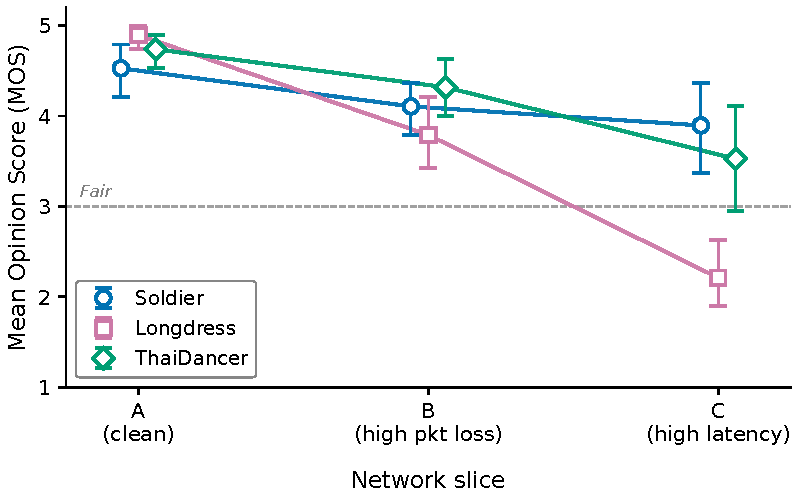
\includegraphics[width=\linewidth]{mosaic-mos.pdf}
    \caption{Mean opinion score with 95\% \gls{ci}.}
    \label{fig:pilot-mos}
  \end{subfigure}\hfill
  \begin{subfigure}[b]{0.49\linewidth}
    \centering
    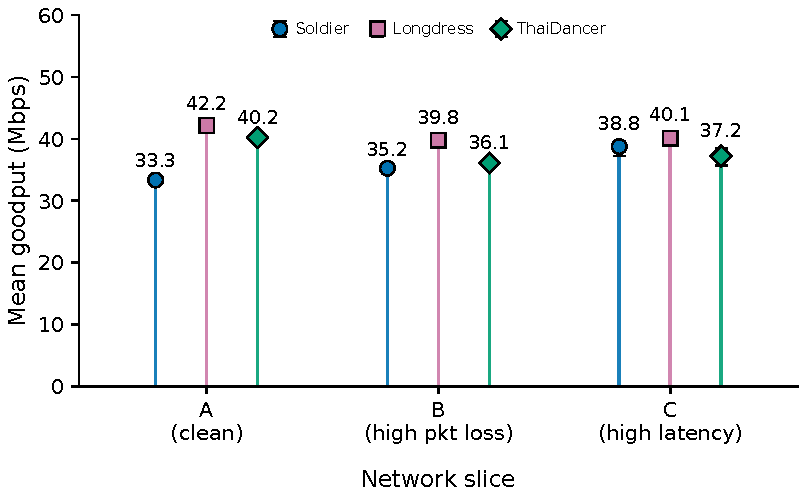
\includegraphics[width=\linewidth]{mosaic-goodput.pdf}
    \caption{Mean application-layer goodput.}
    \label{fig:pilot-goodput}
  \end{subfigure}
  \caption{Three-tier study ($N=20$), per sequence and tier; data
  from~\cite{mosaic2026}.}
  \label{fig:pilot}
\end{figure}

Four lessons shape the present design. Impairment and encoder
configuration were confounded in every tier, so the factorial slices
below hold the encoder fixed. The deadline-miss rate is an incomplete
predictor, so the analysis uses the temporal loss fraction $\tlf$,
which weights each miss by the content it removes. The presentation
order was fixed, so the present study balances it with a Latin square.
And goodput was not the limiting resource, so impairment is applied as
loss and added latency rather than as bandwidth caps.

\subsection{Network Conditions}
\label{sec:design-network}

Four slices share one origin and one renderer
and differ only in the impairment applied at the origin's egress
(Table~\ref{tab:impairments}). Slice~A is the clean reference: no
added loss or latency, \gls{ra} \gof{}=32, the profile an adaptive
service would choose on an unimpaired path, and the slice from which
the ceilings $\qc$ of Eq.~\eqref{eq:ceiling} and the slack $S_k$ of
Eq.~\eqref{eq:slack} are measured. Slices B, C and D form a $2\times2$
factorial on loss and added latency at a fixed encoder, \gls{ldp}
\gof{}=4: B applies loss only, C latency only, and D both at the same
levels, so that the single-factor effects and their combination are
estimated from the same stimuli. A fifth block, E, repeats the D
impairment at \gls{ldp} \gof{}=16 and provides the delivery-unit
contrast of Section~\ref{sec:model-layer1}; it is a separate rating
block rather than a factor, because its purpose is to test the
structural prediction at one operating point, not to map the
\gof\,$\times$\,impairment plane.

The impairment levels are chosen so that each factor alone produces a
measurable but not saturating effect: the loss rate and the added
one-way latency each sit inside the graded region established
in~\cite{mosaic2026}, where mean opinion stayed above the ``Fair''
threshold for most content, and are anchored to the 5G service
performance targets of~\cite{3gpp22261}. Loss is applied as random
(Bernoulli) loss by netem; latency as a fixed one-way delay without
jitter, so that the slack consumed by a unit is deterministic apart
from loss. Loss is accounted for at the IP layer of the origin, and
the renderer's telemetry records, for every unit, the request time,
completion time and deadline outcome, from which $\tlf$ is computed as
in Eq.~\eqref{eq:tlf}.

\begin{table}[t]
  \caption{Impairment slices. All slices share the same origin,
  renderer and casting stage; B--D hold the encoder fixed. \todo{fill
  $p$ and $\ell$}}
  \label{tab:impairments}
  \centering
  \small
  \begin{tabular}{@{}llllll@{}}
    \toprule
    Slice & Loss $p$ & Added latency $\ell$ & Encoder & Role & Rated by \\
    \midrule
    A & 0\%         & \SI{0}{\milli\second}        & \glsentryshort{ra}, \gof{}=32  & clean reference; $\qc$, $S_k$ & all \\
    B & \todo{$p$}  & \SI{0}{\milli\second}        & \glsentryshort{ldp}, \gof{}=4  & loss only & all \\
    C & 0\%         & \todo{$\ell$}                & \glsentryshort{ldp}, \gof{}=4  & latency only & all \\
    D & \todo{$p$}  & \todo{$\ell$}                & \glsentryshort{ldp}, \gof{}=4  & combined & all \\
    E & \todo{$p$}  & \todo{$\ell$}                & \glsentryshort{ldp}, \gof{}=16 & delivery-unit contrast & \todo{subset / all} \\
    \bottomrule
  \end{tabular}
\end{table}

\subsection{Subjective Experiment}
\label{sec:method}

\paragraph{Protocol.}
The study follows ITU-T P.910~\cite{p910} with the \gls{acr} method on
the five-point scale (5~Excellent to 1~Bad); a single-stimulus method
matches how a viewer consumes a stream and needs no reference
presentation inside the headset, unlike the double-stimulus methods of
ITU-R BT.500~\cite{bt500}. The rated attribute is
stated to participants as the \emph{smoothness of playback} of the
figure in front of them, not its visual fidelity; the instruction and
the training clips make the distinction explicit, because the
impairments under test manifest as freezes and frame skips while
spatial quality is fixed within a session
(Section~\ref{sec:model-scope}). Each stimulus is a
\SI{10}{\second} sequence played twice in a row (\SI{20}{\second}),
which exceeds the P.910 recommendation to leave time for \gls{6dof}
exploration without inducing fatigue~\cite{mosaic2026}. A session
opens with a training phase of about \SI{60}{\second} that shows the
three sequences on Slice~A so that the top of the scale is anchored
to the clean presentation, followed by the rated trials: three
sequences $\times$ four slices (A--D) for every participant, plus
block E, in a Latin-square order balanced across participants
so that no slice systematically follows another; this addresses the
fixed presentation order of~\cite{mosaic2026}. Ratings are given
verbally after each trial and entered by the experimenter, keeping
the participant's hands free and the headset on. A session lasts
about \SI{30}{\minute} including briefing and fitting.

\paragraph{Participants and screening.}
\todo{$N = 50$ participants (age range, gender split, prior \gls{vr}
experience), recruited from \anon[the institution]{UNICAMP} and
screened for normal or corrected-to-normal vision and absence of
discomfort during the training phase.} Participants rate in the
headset, standing, free to move within a \SI{2}{\metre} square;
head-tracked viewing is part of the stimulus and is not constrained.
Outlier screening follows ITU-T P.913~\cite{p913}: a participant whose
ratings deviate from the per-condition mean by more than the
prescribed bound in more than a quarter of conditions is excluded
before analysis.

\paragraph{Ethics.}
The protocol was approved by the institutional research ethics
committee through the national platform
(\anon[protocol number withheld for review]{Plataforma Brasil, CAAE
\todo{number}}); participants gave written informed consent, could
stop at any time, and were told they could remove the headset at the
first sign of discomfort. The study complies with the ACM policy on
research involving human participants.

\subsection{Data Processing and Statistical Analysis}
\label{sec:design-analysis}

\paragraph{Opinion scores.}
For each condition (sequence $\times$ slice) we report the mean
opinion score with a bootstrap 95\% \gls{ci} (10,000 resamples over
participants). Because \gls{acr} ratings are ordinal and the
per-condition distributions are not assumed normal, inference is
carried out with a \gls{clmm}: the rating is the ordinal response,
loss (present/absent) and latency (present/absent) are fixed effects
together with their interaction, and participant and sequence are
random intercepts. The two single-factor predictions of
Section~\ref{sec:model-predictions} correspond to the main effects;
the super-additivity prediction corresponds to a positive
loss$\times$latency interaction on the latent scale, and we also
report it on the \mos scale as the contrast
$(\mos_A - \mos_D) - (\mos_A - \mos_B) - (\mos_A - \mos_C)$ with its
bootstrap \gls{ci}. The delivery-unit prediction is the contrast
between blocks D and E at matched impairment.

\paragraph{Transport telemetry and $\tlf$.}
Every rated trial is aligned with the renderer's per-unit log for the
same session, from which the measured temporal loss fraction
$\tlf_{\mathrm{meas}}$ is computed as one minus the ratio of frames
rendered on schedule to frames due, Eq.~\eqref{eq:tlf}. The clean
slice supplies the per-unit slack $S_k$, the base round trip $\rho$
and the goodput $C$; the Layer~1 prediction $\tlf_{\mathrm{pred}}$ is
evaluated from Eqs.~\eqref{eq:recovery}--\eqref{eq:tlf} with the
slice's $(p, \ell)$ and the unit sizes $B_k$ of the bitstream, taking
the expectation over the loss count. Layer~1 is assessed by comparing
$\tlf_{\mathrm{pred}}$ with $\tlf_{\mathrm{meas}}$ per condition.

\paragraph{Model fitting and held-out evaluation.}
Layer~2 is fitted on \emph{measured} $\tlf$: with $\qc$ fixed by
Eq.~\eqref{eq:ceiling} from Slice~A, $\alpha$ is estimated by
non-linear least squares of Eq.~\eqref{eq:crystal} to the
per-condition \mos, and its 95\% \gls{ci} is obtained by bootstrap
over participants. Generalisation is tested by leave-one-out: $\alpha$
is refitted with one slice (or one sequence) withheld and the withheld
condition is predicted without refitting; we report \gls{plcc},
\gls{srocc} and \gls{rmse} on the withheld conditions, pooled. The same
protocol is applied to the five-coefficient regression of
Eq.~\eqref{eq:udora}, refitted on our ratings per sequence, so that
the comparison with the prior model is at equal data and equal
held-out protocol rather than against published figures.
